\cotefile{147}
\scanpage{132}
\mspage{65}
contre il y en a entre $\Pi_{d,d'}$ et $\Pi_d$.
Précisons ce point, en considérant un
morphisme
\[
(215)
\]
\diagram{\begin{tikzcd}[ampersand replacement=\&]\Delta_r\arrow[r,"\alpha"]\&\Delta_{r'}\end{tikzcd}}
\uuline{tel que} $\alpha(0)=0$
alors $D_{\Delta_{r'}}\longrightarrow D_{\Delta_r}$ est un morphisme
étale fini, donc aussi $D^*_{\Delta_{r'}}\unsure{\text{---}|\longrightarrow}D^*_{\Delta_r}$ induit
au dessus de $D^*_{\Delta_r}$) donc on trouve
un diagramme $2$-cartésien (qui \deleted{\unsure{suit|vient}}
\unsure{\inserted{\illegible{1}}}
\deleted{(209)} aussi se déduit de (209)
\[
(216)
\]
\diagram{\begin{tikzcd}[ampersand replacement=\&, column sep=large,row sep=large]
\widetilde\Pi_{\Delta_{r'}}\arrow[r]\arrow[d]\&\widetilde\Pi_{\Delta_r}\arrow[d]\\
\Pi_{\Delta_{r'}}\arrow[r]\&\Pi_{\Delta_r}\arrow[ul,phantom,"2\text{-cart.}" description]
\end{tikzcd}}
)
\margin{Ceci montre que les $\widetilde\Pi_{\Delta_r}\unsure{\longleftarrow|\longrightarrow}\Pi_{\Delta_r}$ et $\widetilde\Pi\unsure{\text{---}|\longrightarrow}\Pi$ sont connus quand on connaît les $\widetilde\Pi_d\longrightarrow\Pi_d$, \unsure{des} projections locales.}
\margin{\deleted{et les $\Pi_d$ \unsure{comme}}
\deleted{\diagram{\begin{tikzcd}[ampersand replacement=\&]\unsure{\Pi_d|P_d}\arrow[r]\&\unsure{G_d|\Pi_d}\end{tikzcd}}}
$D_d^{*!}$ sur $D_{\unsure{d|\Delta}}$
\deleted{\diagram{\begin{tikzcd}[ampersand replacement=\&]{}\arrow[r]\&\unsure{D^*_{\Delta_r}}\end{tikzcd}}}}
où les flèches horizontales induisent sur
les $\pi_1$ des applications injectives à
image d'indice fini (on peut dire que
$\Pi_{\Delta_{r'}}\text{---}\Pi_{\Delta_r}$ fait de $\Pi_{\Delta_{r'}}$ un
rev. fini de $\Pi_{\Delta_r}$).

Toutes ces relations sont encore de
nature essentiellement formelle et triviale,
et marcheraient dans un site quelconque,
sans l'hypothèse spécifique des croisements
normaux, et sans que le remplacement des
\margin{131}

\cotefile{147}
\scanpage{133}
$D_{\Delta_r}$ par les $D^*_{\Delta_r}$, pour définir les
$\Pi_{\Delta_r}$ et $\widetilde\Pi_{\Delta_r}$, \inserted{semble y}
jouer\deleted{\unsure{a|ait}} un rôle particulier.
\inserted{\unsure{et|ici}.}

Pour \uline{$d_0$ fixé}, les systèmes
\diagram{\begin{tikzcd}[ampersand replacement=\&]
\widetilde\Pi_{d_0d_1-d_r}
\arrow[r,phantom,"{\unsure{\text{---}|\longrightarrow}}" description]
\&\Pi_{d_0,-d_r}
\end{tikzcd}}
forment un hom de groupoïdes semi-
simpliciaux, mais de nature \unsure{essent\textsuperscript{lt}|essentiellement}
triviale (il faudrait cepend.\textsuperscript{t} examiner
\unsure{à} l'occasion de plus près cette soi-disant
trivialité -- \unsure{?} elle s'explicite sans peine
en termes de la théorie de Galois
des revêtements de $D^*_{d_0}$ resp. de $P^*_{d_0}$ \unsure{\ldots|--}).

Nous allons maintenant introduire
un élément de structure tout à fait
non-formel, qui ne peut s'obtenir
qu'avec des hypothèses \unsure{de voisinages}
d'intersection normale, et s'exprimant
par le fait que les $\widetilde\Pi_{\Delta_r}$ (NB et
non les $\Pi_{\Delta_r}$ !) forment un groupoïde
$1/2$ simplicial, pour $\Delta_r$ variable. En d'autres
\margin{132}

\cotefile{147}
\scanpage{134}
\mspage{66}

termes, il faut introduire, \deleted{\unsure{des cas}}
pour un morphisme
\diagram{(218)\qquad
\begin{tikzcd}[ampersand replacement=\&]
\Delta_r \arrow[r,no head,"\alpha"] \& \Delta_{r'}
\end{tikzcd},}
un \uline{morphisme correspondant} de groupoïdes
\diagram{(219)\qquad
\fbox{\begin{tikzcd}[ampersand replacement=\&]
\widetilde{\Pi}_{\Delta_{r'}} \arrow[r,"\widetilde{\alpha}^{*}"]
\& \Pi_{\Delta_r}
\end{tikzcd}}}
qu'on appellera l'\uline{hom de générisation}
associé à $\alpha$.
\margin{\figure{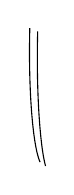
\begin{tikzpicture}
\draw (0,1.7) .. controls (-.02,.9) and (.04,.2) .. (.13,0);
\draw (.10,1.66) .. controls (.08,.9) and (.13,.2) .. (.20,-.05);
\end{tikzpicture}}}
Comme $\alpha$ se factorise
canoniquement en un hom surjectif
suivi d'un hom injectif de simplexes,
on est ramené à examiner séparément
les deux cas. Mais si $\alpha$ est surjectif
(``hom de dégénérescence''), \deleted{l'homomorphisme}
\inserted{on a $\alpha(0)=0$}
donc on est dans le cas déjà envisagé --
\deleted{\unsure{correspondant}}\inserted{d'ailleurs} dans ce cas
\diagram{\begin{tikzcd}[ampersand replacement=\&]
D^*_{\Delta_{r'}} \arrow[r] \& D^*_{\Delta_r}
\end{tikzcd}}
\unsure{se} décompose en des morphismes \unsure{:|;}
\diagram{(220)\qquad
\begin{tikzcd}[ampersand replacement=\&]
D^*_{d'_0,\unsure{\ldotp-\!-|-\!-},d'_{r'}}
\arrow[r] \&
D^*_{\unsure{d_0^{\deleted{\prime}}|d_0^*},-\!-,\unsure{d_r^{\deleted{\prime}}|d_r^*}}
\end{tikzcd},}
$(d_0,-\!-,d_r)$ est déduite de $(d'_0,-,d'_r)$
en \unsure{réécrivant} cette suite, en répétant certains
de ses éléments -- et \deleted{les} alors (220) est
un iso -- donc \uline{si $\alpha$ est un hom}
\margin{On voit que la considération des
$\widetilde{\Pi}_{d_0-d_r}$, $\Pi_{d_0,-d_r}$
pour $d_0,-\!-,d_r$ \unsure{non}
\unsure{\uline{strictement}|\uuline{strictement}}
décroissants, et celle de $\alpha^*$, pour $\alpha$
\unsure{non} \uline{stricts} croissants,
est de la poudre aux yeux, simplement !}
\margin{133}

\cotefile{147}
\scanpage{135}
\uline{de dégénérescence}, \uline{alors} (219) \uline{est un}\deleted{e}
\deleted{\unsure{équiv.}}\uline{isomorphisme}, de nature ess.\textsuperscript{t} triviale.

On est donc réduit à regarder le
cas d'une application \uline{injective} $\alpha$ (``opération
face''), et le \inserted{seul} cas qui \deleted{\unsure{pose}} pose problème
est bien sûr celui où $\alpha(0)\ne0$. Donc
\[
\tag{221}
\left\{\begin{aligned}
d_*&=\{d_0>d_1\cdots>d_r\},\quad\text{et si}\\
d'_*&=\{d'_0>d'_1>{-}>d'_{r'}\}\text{ est }
\text{\deleted{\unsure{une sous-suite}}}\inserted{\text{contenu dans }d_*},
\end{aligned}\right.
\]
$d'_0\ne d_0$ i.e. $d'_0<d_0$, il faut
\par\noindent définir l'hom
\diagram{\begin{tikzpicture}
\node (map) at (0,0) {\begin{tikzcd}[ampersand replacement=\&,column sep=2.8cm]
\Pi_1P^*_{d_0\deleted{\unsure{\geq}}d_1,\unsure{-\,-|\ldots},d_r}\arrow[r]\&
\Pi_1P^*_{d'_0,-,d'_r}
\end{tikzcd}};
\node[anchor=east] at (map.west) {$(222)$};
\node[anchor=south west,align=left,font=\footnotesize] at (1.1,0.75)
{attention, on a\\subrepticement changé\\de notations, en interver-};
\node[anchor=north west,align=left,font=\footnotesize] at (1.1,-0.8)
{tissant $d_*$ et $d'_*$ !};
\draw (2.1,2.15) .. controls (1.1,1.95) and (0.6,1.35) .. (0.75,0.65)
.. controls (1.6,0.55) and (4.65,0.65) .. (5.0,0.45)
.. controls (5.25,0.15) and (5.25,-0.3) .. (5.1,-0.5)
.. controls (4.3,-0.55) and (2.95,-0.4) .. (2.1,-0.55);
\draw (1.65,-0.7) .. controls (0.65,-0.85) and (0.8,-1.4) .. (1.55,-1.5)
.. controls (2.6,-1.6) and (4.4,-1.25) .. (5.0,-1.2);
\end{tikzpicture}}
\margin{on se réduit au cas de $d_0,d_1,-,d_r$ strict.\textsuperscript{t} décroissants -- auquel \unsure{on} parvient aussitôt\unsure{. --|.} En fait, on est ramené au cas où $r'=r-1$, et où il s'agit de l'opération ``face de codim $1$'' pour laquelle $\alpha(0)\ne0$, donc correspondant :
\diagram{\begin{tikzcd}[ampersand replacement=\&]D_{d_0,d_1,-,d_r}\arrow[r]\&D_{d_1,-,d_r}\end{tikzcd}}}

Notons que l'on a
\diagram{$(223)\qquad$\begin{tikzcd}[ampersand replacement=\&]
D^{\deleted{*}}_{d_0,\unsure{-\,-|\ldots},d_r}\arrow[r]\&D_{d'_0,-,d'_{r'}}
\end{tikzcd}}
(mais \uline{non} un morphisme entre les
espaces avec $*$ !), qui est une immersion \inserted{locale}
d'espaces analytiques lisses, de codim
$d_0-d'_0$, \deleted{qui}\inserted{\unsure{ainsi|et}} s'insère dans le diagramme
\margin{134}

\cotefile{147}
\scanpage{136}
\mspage{67}
\diagram{$(22\deleted{\unsure{?}}4)\qquad$\begin{tikzcd}[ampersand replacement=\&]
D_{d_0,-,d_r}\arrow[r]\arrow[d]\&D_{d'_0\,--\,d'_{r'}}\arrow[d,no head]\\
D_{d_0,d'_0}\arrow[r]\&D_{d'_0}^{\deleted{\unsure{*}}}
\end{tikzcd}}
où les flèches verticales sont étales,
et la $2^{\mathrm{ième}}$ flèche horizontale est une
immersion locale de codim $d_0$\deleted{$\unsure{-}d'_0$. \unsure{On a}}
\[
\tag{225}\unsure{d|\delta}=d_0-d'_0
\]
[Dans le typique (auquel on se réduit)
où $\unsure{\{}d'_* = \{\uline{d_1}>-- >d_r\}$, le diagramme
(224) est cartésien -- \deleted{\unsure{comme on voit}}\inserted{plus \unsure{gén.\textsuperscript{t}|génér.\textsuperscript{t}}}, il
\unsure{reste} \deleted{\unsure{tjs}} cartésien, \inserted{si $d'_0=d_1$} et c'est trivial.]
\margin{\uline{NB} Dans le cas général, on a
\diagram{\begin{tikzcd}[ampersand replacement=\&, column sep=small]
D_{d_*}\arrow[r,"{\text{fini étale}}"']\arrow[dd,dotted]\&D_{\widetilde d'_*}\arrow[r]\arrow[d]\&D_{d'_*}\arrow[d]\\
\&D_{d_0,d'_0}\arrow[dl,dotted]\arrow[r,no head]\&D_{d'_0}\\
D_{d_0}\&\&
\arrow[ul,phantom,from=2-3,to=1-2,"{\text{cart}}" description]
\end{tikzcd}}}
Considérons le morphisme induit
\diagram{$(225)\qquad$\begin{tikzcd}[ampersand replacement=\&]D^*_{d_*}\arrow[r]\&D_{d'_*}\end{tikzcd}}
(Attention, on a mis un $*$ en exposant
à $D_{d_*}$ seulement, non : $D_{d'_*}$ !).

Nous munissons $D_{d'_*}$ du diviseur
$\Theta_{d'_*}$ image inverse de $\Theta_{d_0}$ sur $D_{d_0}$.
On désigne par $\Theta_{d'_*}^{(p)}$ le ``squelette
de dim $p$'' de $\Theta_{d'_*}^{p}$, et \deleted{\unsure{p}} on pose
\margin{135}

\cotefile{147}
\scanpage{137}

\[
(226)\qquad
\Theta_{d'_*}^{\unsure{d}*}\overset{\mathrm{def}}=
\Theta_{d'_*}^{\unsure{d}}\setminus
\Theta_{d'_*}^{\unsure{d+1|d1}}
\]
squelette ``privé'' de codim. $d$ de
$\Theta_{d'_*}$ dans $D_{d'_*}$.

Ceci posé, on sait que $225$ \unsure{\uline{induit}}
un \deleted{morphisme} \uline{isomorphisme local}
\uline{de} $D_{d_*}$ \uline{sur}
\deleted{$\unsure{D_{d'_*}|\Theta_{d'_*}}$}
$\Theta_{d'_*}^{d*}$. Plus
précisément, \deleted{$\Theta_{d'_*}^{d*}$ s'identifie \unsure{à} :}
\deleted{$\unsure{D_{(d_0,d'_0,-,d'_r)}}\ \unsure{:|.}\
D_{\widetilde d'_*}$, \unsure{où}}
\diagram{(22\unsure{7})\qquad
\begin{tikzcd}[ampersand replacement=\&]
\Theta_{d'_*}^{(d)} \&
D_{\widetilde d'_*}\arrow[l,"\sim"']
\end{tikzcd}}
où \deleted{$d$}
\[
\widetilde d'_*=(d_0,d'_0,-\!-,d'_r)
\]
et cet isom. induit un isom
\diagram{(228)\qquad
\begin{tikzcd}[ampersand replacement=\&]
D_{\widetilde d'_*}^{*}\arrow[r,"\sim"]\&
\Theta_{d'_*}^{(d)*},
\end{tikzcd}}
d'autre part (223)
$D_{d_*}\mathrel{\text{---}}D_{d'_*}$ se
factorise en
\diagram{(229)\qquad
\begin{tikzcd}[ampersand replacement=\&]
D_{d_*}\arrow[r,no head]\&
D_{\widetilde d'_*}\arrow[r]
\arrow[d,phantom,"\rotatebox{90}{$\simeq$}" description]\&
D_{d'_*}\\
\&\Theta_{d'_*}^{(d)\unsure{*}}\&
\end{tikzcd}}
donc c'est un morphisme étale fini,
suivi \inserted{est} \unsure{d'un|\deleted{d'un}} morphisme d'inclusion de
$\Theta_{d'_*}^{(d)}$ dans $D_{d'_*}$. De plus, comme $D_{d_*}^{*}$ est
\margin{136}

\cotefile{148}
\scanpage{2}

\margin{(29.11.83)}

Soit $X$ surf. à bord compacte orientée, à
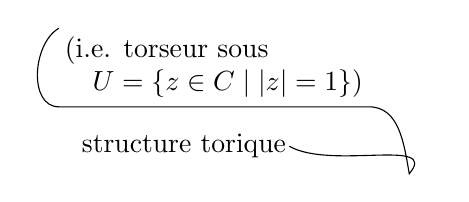
\begin{tikzpicture}[baseline=(torique.base)]
\node[anchor=west,inner sep=1pt] (torique) at (0,0) {structure torique};
\node[anchor=south west,inner sep=2pt,align=left] (torusnote) at (-.25,.5)
{\inserted{\begin{tabular}{@{}l@{}}(i.e. torseur sous\\
\quad$\mathbb U=\{z\in\mathbb C\mid |z|=1\}$)\end{tabular}}};
\draw (torusnote.north west) to[out=210,in=180] (torusnote.south west)
 -- (torusnote.south east) to[out=0,in=100] (4.2,-.35)
 to[out=50,in=-30] (torique.east);
\end{tikzpicture}
donnée sur les comp. connexes du bord.
On définit

\[
\begin{aligned}
\operatorname{SRT}(\unsure{X})={}&
\text{quotient du groupe des autom de }X
\text{ (\deleted{\unsure{en}} resp. l'orientation}\\
&\text{et les structures toriques) par la comp. neutre du}\\
&\text{sous-groupe }\operatorname{Aut}^!(\vec X)
\deleted{\unsure{\mathrm{bijec.}}}
\text{ de Aut qui induit}\\
&\text{l'identité sur }\partial X
\end{aligned}
\]

On a ainsi un dévissage de $\operatorname{SRT}(X)$ en trois étages

\[
\underbrace{S_{\unsure{*}}T^!(X)}_{
\operatorname{Aut}^!(\unsure{\vec X|\overline X})/
\text{comp. neutre}}
\qquad\mathbb U^I\qquad\unsure{\mathfrak S_I}
\qquad I=\pi_0(\partial X)
\]

ou encore

\[
\mathbb Z^I\qquad T(X)\qquad\mathbb U^I\qquad\unsure{\mathfrak S_I}
\]

En fait, on définit can! un sous-groupe
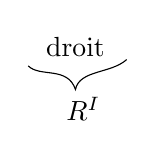
\begin{tikzpicture}[baseline=(ri.base)]
\node[inner sep=1pt] (ri) at (0,0) {$\mathbb R^I$};
\node[anchor=south] at (-.1,.55) {\inserted{droit}};
\draw (-.7,.55) .. controls (-.55,.4) and (-.2,.55) .. (-.1,.25)
 .. controls (-.05,.5) and (.35,.45) .. (.55,.63);
\end{tikzpicture}
de $\operatorname{SRT}(X)$
contenant $\mathbb Z^I$, de telle façon qu'on ait

\[
\underbrace{\operatorname{SRT}^!(X)}_{
\substack{\text{noyau de}\\
\operatorname{SRT}^!(\alpha)\to\unsure{\mathfrak S_I'|\mathfrak S_I^!}}}
=\mathbb R^I.S_*T^!(X)
\]

\diagram{
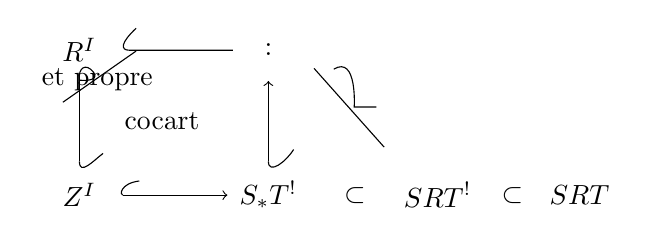
\begin{tikzpicture}[x=1cm,y=1cm]
\node (r) at (0,1.85) {$\mathbb R^I$};
\node (z) at (0,0) {$\mathbb Z^I$};
\node (p) at (2.4,1.85) {$\mathord{:}$};
\node (st) at (2.4,0) {$S_*T^!$};
\node at (3.5,0) {$\subset$};
\node at (4.55,0) {$\operatorname{SRT}^!$};
\node at (5.5,0) {$\subset$};
\node at (6.35,0) {$\operatorname{SRT}$};
\draw (.72,2.12) .. controls (.53,1.94) and (.51,1.84) .. (.64,1.84)
 -- (1.95,1.84);
% The upper end of this left stroke merges with cancelled lettering and a diagonal.
\draw (0,.43) -- (0,1.46);
\draw (0,1.46) .. controls (-.02,1.61) and (.08,1.69) .. (.18,1.56)
 .. controls (.24,1.47) and (.13,1.45) .. (0,1.46);
\draw (-.21,1.18) -- (.72,1.83);
\node[anchor=east] at (-.24,1.62) {$\unsure{\phantom{\uparrow}}$};
\draw (0,.43) .. controls (.0,.24) and (.18,.44) .. (.3,.53);
\node[anchor=west] at (.45,.94) {cocart};
\node[anchor=west] at (-.6,1.47) {\deleted{\unsure{et propre}}};
\draw[->] (.55,0) -- (1.88,0);
\draw (.76,.18) .. controls (.52,.15) and (.51,.0) .. (.55,0);
\draw[->] (2.4,.43) -- (2.4,1.45);
\draw (2.4,.43) .. controls (2.4,.25) and (2.63,.43) .. (2.72,.58);
% The following two source strokes have an unresolved reading (lambda / crossed 2).
\draw (2.98,1.61) -- (3.87,.61);
\draw (3.23,1.6) .. controls (3.53,1.78) and (3.49,1.12) .. (3.49,1.12)
 -- (3.77,1.12);
\node[anchor=west] at (3.91,1.12) {$\unsure{\phantom{\lambda}}$};
\end{tikzpicture}
}

i.e. on a

\margin{\uline{NB} $\operatorname{SUT}(X)\simeq
T(X)\times_{\unsure{\mathfrak S_I}}\operatorname{Aut}((T_i)_{i\in I})$}

\margin{Jusqu'ici on ne fait intervenir
que $S_*T^!(X)$, à l'exclusion de $S_*T(X)$,
dont la défini. exige une str. suppl.
$\uline{s}$, cf ci-dessous}

\diagram{
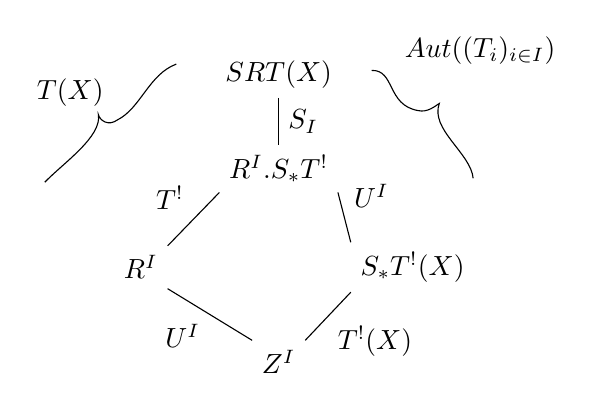
\begin{tikzpicture}[x=1cm,y=1cm]
\node (top) at (0,2.45) {$\operatorname{SRT}(X)$};
\node (mid) at (0,1.25) {$\mathbb R^I.\unsure{S_*T^!}$};
\node (left) at (-1.75,0) {$\mathbb R^I$};
\node (right) at (1.7,0) {$S_*T^!(X)$};
\node (bottom) at (0,-1.2) {$\mathbb Z^I$};
\draw (top.south) -- (mid.north) node[midway,right] {$\unsure{\mathfrak S_I}$};
\draw (mid.south west) -- (left.north east) node[midway,above left] {$T^!$};
\draw (mid.south east) -- (right.north west) node[midway,above right] {$\mathbb U^I$};
\draw (left.south east) -- (bottom.north west) node[midway,below left] {$\mathbb U^I$};
\draw (bottom.north east) -- (right.south west) node[midway,below right] {$T^!(X)$};
\draw (-1.3,2.58) .. controls (-1.65,2.45) and (-1.75,2.02) .. (-2.05,1.87)
 .. controls (-2.16,1.79) and (-2.27,1.86) .. (-2.29,1.94)
 .. controls (-2.24,1.66) and (-2.74,1.32) .. (-2.97,1.08);
\node[anchor=east] at (-2.1,2.22) {$T(X)$};
\draw (1.18,2.5) .. controls (1.48,2.51) and (1.37,2.06) .. (1.77,1.99)
 .. controls (1.89,1.96) and (1.99,2.05) .. (2.04,2.08)
 .. controls (1.92,1.75) and (2.44,1.45) .. (2.47,1.13);
\node[anchor=south west] at (1.48,2.45) {$\operatorname{Aut}((T_i)_{i\in I})$};
\end{tikzpicture}
}

d'où
\diagram{
\begin{tikzpicture}[x=1cm,y=1cm]
\node (quot) at (0,0) {$\operatorname{SRT}\deleted{(X)}/\mathbb Z^I
 \overset{\text{déf}}=\operatorname{SUT}(X)$};
\node (prod) at (-.85,-1.1) {$T^!(X)\times\mathbb U^I$};
\draw[->] (-1.2,-.3) -- (-1.2,-.78);
\node at (1.42,-.62) {$\Big\}\ \unsure{\mathfrak S_I}$};
\draw (-3.0,-1.52) .. controls (-2.4,-1.6) and (-2.0,-1.54) .. (-1.62,-1.51)
 .. controls (-1.44,-1.71) and (-.92,-1.6) .. (-.4,-1.51)
 .. controls (.13,-1.64) and (.48,-1.64) .. (1.1,-1.45)
 .. controls (1.52,-1.41) and (1.85,-1.47) .. (2.0,-1.47);
\end{tikzpicture}
}

\[
(*)\qquad1\longrightarrow\mathbb U^I\longrightarrow
\operatorname{SUT}(X)\longrightarrow
\unsure{\deleted{\mathfrak S}T|T}(X)-1
\]

De plus, chaque fois qu'on se donne un
marquage, i.e. un pt \deleted{\unsure{de}}

\[
\uline{s}=(s_i)\in
\prod_{i\in I=\pi_0(\partial X)}
\deleted{\unsure{\mathbb U_i}}T_i
\]

\margin{$T_i=$ comp. connexe (torique) de
$\partial X$ d'indice $i$\par\hspace{1.1cm}$\unsure{i}$}

on trouve un plongement
\[
S_*T^{\deleted{\unsure{!}}}(X,\uline{s})\hookrightarrow\operatorname{SRT}(X)
\]
tel qu'on en \unsure{déduise|déduire}

\[
S_*T^{\deleted{\unsure{!}}}(X,\uline{s})
\mathbin{\wedge}_{\mathbb Z^I}\mathbb R^I
\simeq\operatorname{SRT}(X)
\]

\margin{1}

\cotefile{148}
\scanpage{3}

Une façon de le voir est de dire que
la donnée de $\uline{s}$ définit un scindage
\inserted{$\varphi_{\uline{s}}$} de
l'extension $(*)$ ci-dessus, et que \unsure{vu pour}
ss-groupe de $\operatorname{SRT}(X)$,
$S_1T(X,\uline{s})$ s'identifie
à l'image inverse de
\[
\varphi_{\uline{s}}(T(X))\subset\operatorname{SUT}(X)
\]
par l'hom. can
$\operatorname{SUR}(X)\mathrel{\unsure{\text{---}|\longrightarrow}}\operatorname{SUT}(X)$
de passage au quotient. Le chgt de
$\uline{s}$ en $\uline{s}'=u.\uline{s}$
transforme $\varphi_{\uline{s}}$ en
\[
\varphi_{\uline{s}'}=\operatorname{int}(u)\circ\varphi_{\uline{s}}
\]
donc (si $\widetilde u\in\mathbb R^I$ relève $u$) on trouve
\[
S_1T(X,\uline{s}')
=\operatorname{int}(\widetilde u)S_1T(X,\uline{s})\unsure{.|,}
\]

En termes de $\unsure{\overline X|\vec X}$, la définition de
$S_1T(X,\uline{s})$
dépend un choix $\uline{s}$ \uline{non-anodin},
par contre celle de $S_1RT(X)$ ne dépend que d'
un choix anodin, celui de la famille des
structures toriques $(t_i)_{i\in I}$.
De plus $\prod T_i$ comme
torseur sous $\unsure{\mathbb U^I}$ se réalise
\inserted{(pas fidèlement d'ailleurs)}
comme \unsure{une classe} de scindages de l'ext. $(*)$
(via autom. int. par $\mathbb U^I$)
$\bigl[$déduits de $\operatorname{SRT}(X)$
avec les structures suppl.$\bigr\}$
savoir\unsure{)|,} les inclusions

\diagram{
\begin{tikzcd}[ampersand replacement=\&,row sep=small,column sep=small]
\mathbb R^I\arrow[dr,bend right=12] \&\\
\&\operatorname{SRT}(X)\\
S_1T^!(X)\arrow[ur]\&
\end{tikzcd}
}

\unsure{coïncid.|coïncidant} sur $\mathbb Z^I$.

\margin{2}

\cotefile{148}
\scanpage{4}

Ceci dit, si on se donne un
multimarquage de $\partial X$, savoir pour
chaque $i\in I$ un $n_i\in\mathbb N^*$ et un
sous-\inserted{\unsure{$\mathbb Z_{n_i}$|$\mathbb Z/n_i$}-}torseur
$T_i(n_i)\subset T_i$,
\deleted{\unsure{les groupes|de groupe}} i.e
un $s_i\in T_i^{\wedge n_i}$, d'où
$\deleted{\unsure{\uline{s}\in}}$
\[
\uline{s}\in\prod_{i\in I}T_i^{\wedge n_i},
\]
alors le groupe de Teichmüller multimarqué
$S_{\unsure{*|1}}T(\unsure{X},\uline{s})$,
généralisant le précédent, est
plongé dans $\operatorname{SRT}(X)$ de façon naturelle,
en prenant un $s_i^0$ dans chaque $T_i(n_i)$, d'où
$\uline{s}^0\in\prod T_i$ et
$ST(X,\uline{s}^0)\subset\operatorname{SRT}(X)$,
et on prend le ss-groupe
\[
ST(X,\uline{s})=ST(X,\uline{s}^0).
\prod_{i\in I}\frac1{n_i}\mathbb Z_i
\]
où $\mathbb Z_i$ est le $i$ème facteur de
$\mathbb Z^I\subset\operatorname{SRT}(X)$.

\margin{3}
